\documentclass[
%  draft,
  10pt,
  a4paper,
  parskip,
  titlepage,
%  twocolumn,
%  twoside,
%  openright,
%  listof=totocnumbered,
%  bibliography=totocnumbered,		% Literaturverzeichnis im Inhaltsverzeichnis aufführen und nummerieren
%  liststotoc,				% Verzeichnisse im Inhaltsverzeichnis aufführen
%  idxtotoc				% Index im Inhaltsverzeichnis aufführen
]{scrartcl}
%]{report}
%]{scrbook}

\usepackage{graphics}
\usepackage{epstopdf}
\usepackage[utf8]{inputenc}
\usepackage[english]{babel}
\usepackage{csquotes}
\usepackage{amsmath}
\usepackage{amsfonts}
\usepackage{rotating}
\usepackage{float}
\usepackage{amssymb}
\usepackage[svgnames]{xcolor}
\usepackage{tikz}
\usepackage{listings}
\usepackage[breaklinks]{hyperref}
\usepackage[all]{hypcap}        % jump to the start of table/figure instead to the caption of it (fix for hyperref)
%\usepackage{url}
\usepackage{placeins}           % for \FloatBarrier
\usetikzlibrary{arrows,positioning,shapes} 
\usepackage{titlepage}
\usepackage{textcomp} % for \textgreater and \textless
\usepackage{comment}
\usepackage{caption}
\usepackage{subcaption}
\usepackage{xcolor}
\usepackage{chngpage}
\usepackage{multirow}

\usepackage{fancyhdr}
\pagestyle{fancy}
\fancyhead[LO,RE]{\iffloatpage{}{Report: Analysis of a Messaging System}}
\fancyhead[RO,LE]{\iffloatpage{}{\thepage}}
\fancyfoot{}
\renewcommand{\headrulewidth}{\iffloatpage{0pt}{0.4pt}}

\lstset{ %
  basicstyle=\footnotesize,       % the size of the fonts that are used for the code
  numbers=left,                   % where to put the line-numbers
  numberstyle=\tiny\color{gray},  % the style that is used for the line-numbers
  numbersep=5pt,                  % how far the line-numbers are from the code
  backgroundcolor=\color{white},  % choose the background color. You must add \usepackage{color}
  showspaces=false,               % show spaces adding particular underscores
  showstringspaces=false,         % underline spaces within strings
  showtabs=false,                 % show tabs within strings adding particular underscores
  frame=single,                   % adds a frame around the code
  rulecolor=\color{black},        % if not set, the frame-color may be changed on line-breaks within not-black text (e.g. commens (green here))
  tabsize=2,                      % sets default tabsize to 2 spaces
  captionpos=b,                   % sets the caption-position to bottom
  breaklines=true,                % sets automatic line breaking
  breakatwhitespace=false,        % sets if automatic breaks should only happen at whitespace
  escapeinside={\%*}{*)},         % if you want to add a comment within your code
  morekeywords={*,...}            % if you want to add more keywords to the set
}


\setcounter{tocdepth}{5}   
\setcounter{secnumdepth}{5} 

\author{Thomas Frick (LEGI)\\Matthias Ganz (LEGI)\\Philipp Rohr (04-397-030)}

\makeatletter
\AtBeginDocument{\markboth{\@author}{\@title}}   % gives access to those variables through \@author

\title{Implementation of a Virtual File System}
\date{\today}

\hypersetup
{
  pdftitle={\@title},
  pdfauthor={\@author},
  pdfsubject={}
}

\clubpenalty=10000
\widowpenalty=10000\displaywidowpenalty=10000 

\newcommand{\code}[1]{\texttt{#1}}
\newcommand{\console}[1]{\fbox{\texttt{#1}}}
\newcommand{\file}[1]{\textsl{#1}}

\newcommand{\anmerkung}[1]{\marginpar{\color{red}\footnotesize{#1}}}
\newcommand{\todo}[1]{{\color{red}#1\index{todo!#1}}\anmerkung{{\color{red} todo}}}



\setcounter{tocdepth}{2}
\begin{document}
\maketitle

\tikzstyle{app}=[anchor=center,minimum width=3 cm,minimum height=2 cm,rectangle,rounded corners,draw=black, top color=white, bottom color=blue!30,very thick, text centered]
\tikzstyle{map}=[anchor=center,minimum width=1 cm,minimum height=1 cm,rectangle,rounded corners,very thick, text centered,draw=black,fill=white]
\tikzstyle{event}=[map, fill=green!30,very thick, text centered]
\tikzstyle{arrow}=[->,thick]
\tikzstyle{derive}=[->, >=open triangle 90, thick]

\tikzstyle{use}=[<-, >=open diamond, thick]
\tikzstyle{need}=[<-, >=diamond, thick]

\tikzstyle{Interface}=[rectangle,draw=black, fill=yellow!60,rotate=90]
\tikzstyle{file}=[anchor=center,draw=black, top color=white, bottom color=yellow!30,thick, text centered]

\tikzstyle{class}=[anchor=center,draw=black, fill=yellow!30, thick, rectangle split, rounded corners, rectangle split parts=3, align=left]

\tikzstyle{page}=[anchor=center,minimum width=1 cm,minimum height=1 cm,rectangle, thick, text centered,draw=black,fill=white]
\tikzstyle{label}=[anchor=center,text centered]

\tikzstyle{physical}=[fill=yellow!30]
\tikzstyle{virtual}=[fill=blue!60]
\tikzstyle{org}=[fill=blue!10]



\setcounter{secnumdepth}{3}
\setcounter{tocdepth}{3}
\tableofcontents

\begin{abstract}
\section*{Abstract}
The \textit{Virtual File System} was implemented during the course
\textit{Java and C\# in depth}.

This version of the document describes the project at the final state of
milestone 1. and so on\ldots
 
\end{abstract}


\section{The Full Model}
After we did one more experiment that is explained in the appendix
 I could could examine the measured values and made some observations that are
  described in this section. Based on those observations I built the full model
   that will be the basis of a mean value analysis shown further in the document.

\subsection{Definitions}
blablab

\subsection{Observations}
This is a table (table \ref{table:measuredData}) measured throughout the
 and a footnote \footnote{Described in the appendix \ref{sec:client_scale_out}} 
 
\begin{table}[h!]
 \centering
 \begin{tabular}{| r| rrrr | rr | r |}
    \hline \textbf{$N$} & \textbf{$R_{puts}$} & \textbf{$R_{retrieves}$} & \textbf{$R_{meas}$} & \textbf{$X_{meas}$} & \textbf{$X_{calc}$} & \textbf{$R_{calc}$}  & \textbf{$Z_{calc}$} \\
    \hline 32  & 69  & 112 & 181 & 176.5 & 176.8 & 181 & 0 \\
    \hline 64  & 72  & 113 & 185 & 344.7 & 345.9 & 186 & 1 \\
    \hline 96  & 81  & 115 & 196 & 486.4 & 489.8 & 197 & 1 \\
    \hline 128 & 98  & 119 & 217 & 586.8 & 589.9 & 218 & 1 \\
    \hline 160 & 124 & 130 & 254 & 628.3 & 629.9 & 255 & 1 \\
    \hline 192 & 161 & 156 & 317 & 603.9 & 605.7 & 318 & 1 \\
    \hline 224 & 213 & 204 & 417 & 536.4 & 537.2 & 418 & 1 \\
    \hline 256 & 251 & 230 & 481 & 531.2 & 532.2 & 482 & 1 \\ 
    \hline
 \end{tabular}
\caption{Measured (on client side) and calculated data of the whole system.}
\label{table:measuredData}
\end{table}


\subsection{The Model}
and a figure \ref{fig:full_model}.  fancy foobar

\begin{figure}[h!]
\centering
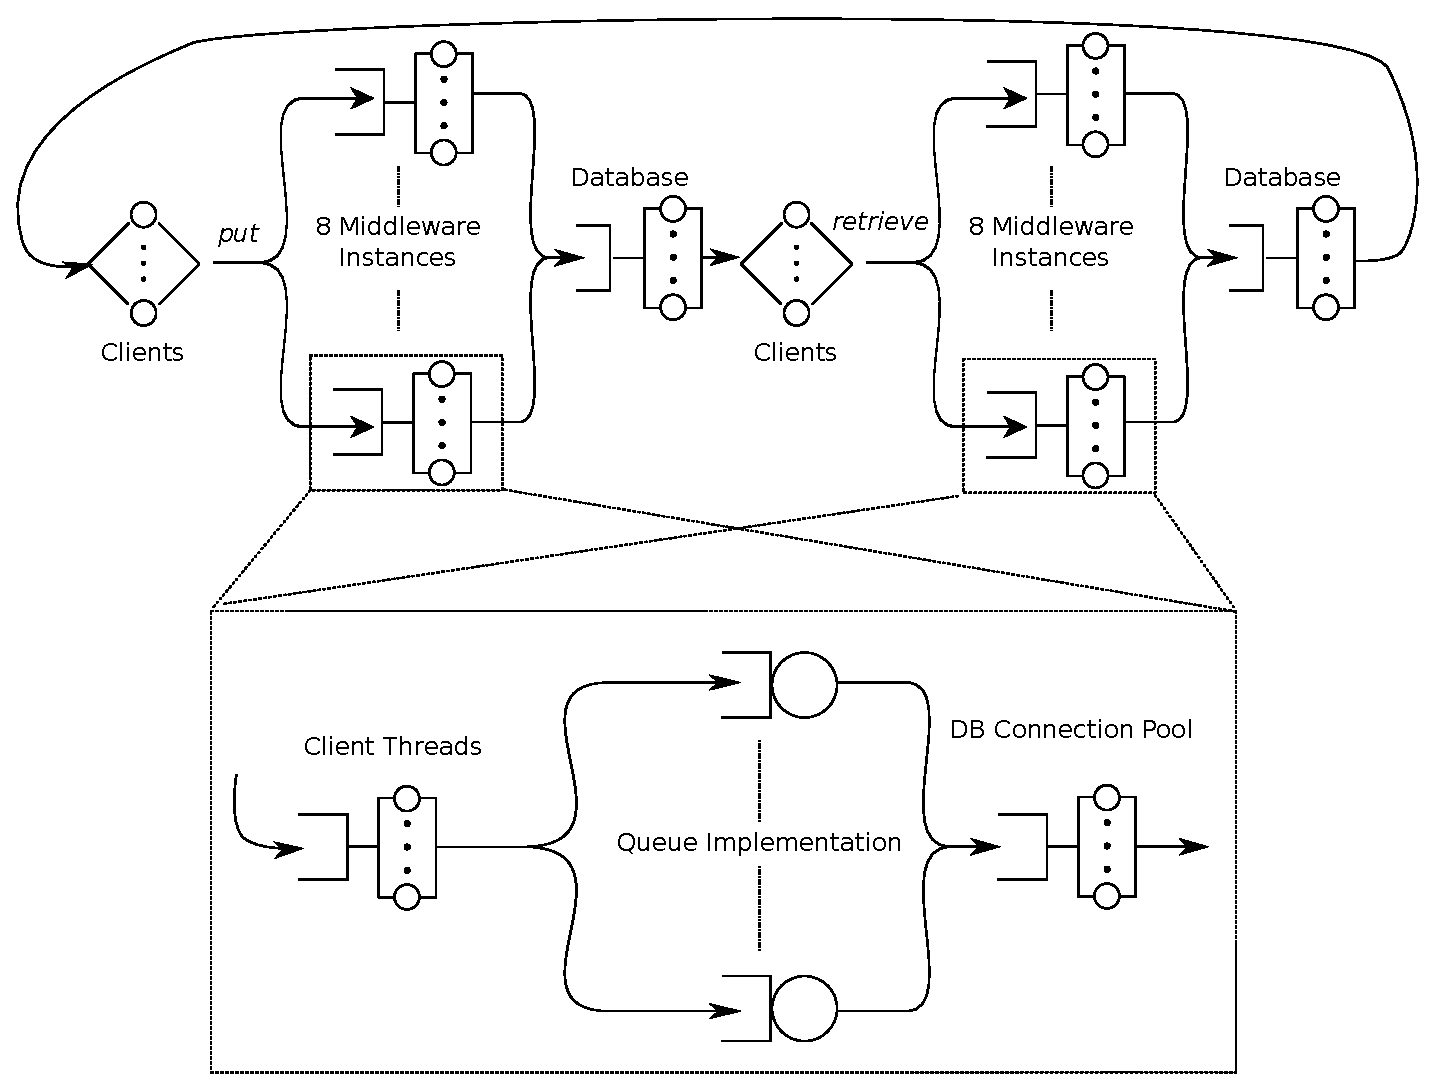
\includegraphics[width=1\textwidth]{figures/full_model.eps}
\caption{Full model of the system.}
\label{fig:full_model}
\end{figure}

\newpage

citation\cite{Raj}. 

some math

\[\mu(n) =
\left\{
	\begin{array}{ll}
		n/S  & \mbox{if } n=1,2,...,m-1 \\
		m/S & \mbox{if } n=m,m+1,...,\infty
	\end{array}
\right.
 \]




\section{Glossary}


\paragraph{Virtual Disk} A virtual disk denotes a container file that is stored
on the host file system. A virtual disk can be opened with the software that is
developed during this project and stores the actual files. The file extension of
the virtual disk is ``*.bfs''.




\listoffigures
\listoftables

\bibliographystyle{plain}
\bibliography{literature}
\end{document}
